%!TEX program = xelatex
% 完整编译: xelatex -> biber/bibtex -> xelatex -> xelatex
\documentclass[lang=cn,a4paper,citestyle=gb7714-2015, bibstyle=gb7714-2015]{elegantpaper}

\title{NSGA-II算法}

\author{姜孟冯 \\中国矿业大学 / 应急管理部信息研究院}

\date{\zhtoday}

%%%%%%%%%%%%%%%%%%%%%%%%%%%%%%%%%%%%%%%%%%%%%%%%%%%%%%%%%%%%%%%%%%%%%
% PACKAGES                                                          %
%%%%%%%%%%%%%%%%%%%%%%%%%%%%%%%%%%%%%%%%%%%%%%%%%%%%%%%%%%%%%%%%%%%%%
\usepackage{amssymb}
\usepackage{optidef}
\usepackage{tabularray}
\usepackage{biblatex}
\addbibresource[location=local]{reference.bib} % 参考文献
\usepackage{graphicx}
%%%%%%%%%%%%%%%%%%%%%%%%%%%%%%%%%%%%%%%%%%%%%%%%%%%%%%%%%%%%%%%%%%%%%%
% STYLE ENVIRONMENT                                                  %
%%%%%%%%%%%%%%%%%%%%%%%%%%%%%%%%%%%%%%%%%%%%%%%%%%%%%%%%%%%%%%%%%%%%%%

%%%%%%%%%%%%%%%%%%%%%%%%%%%%%%%%%%%%%%%%%%%%%%%%%%%%%%%%%%%%%%%%%%%%%%
% MY COMMANDS                                                        %
%%%%%%%%%%%%%%%%%%%%%%%%%%%%%%%%%%%%%%%%%%%%%%%%%%%%%%%%%%%%%%%%%%%%%%
\newcommand{\R}{\mathbf{R}}
\newcommand{\C}{\mathbf{C}}
\newcommand{\F}{\mathbf{F}}
\newcommand{\U}{\mathit{U}}
\newcommand{\V}{\mathit{V}}
\newcommand{\W}{\mathit{W}}
\newcommand{\poly}{\mathcal{P}}
\newcommand{\espace}{\mathcal{L}}
\newcommand{\expect}{\mathcal{E}}
\newcommand{\mat}{\mathcal{M}}
\newcommand{\mtxA}{\mathcal{A}}
\DeclareMathOperator{\Span}{span}
\DeclareMathOperator{\Real}{Re}
\DeclareMathOperator{\Imag}{Im}
\DeclareMathOperator{\Null}{null}
\DeclareMathOperator{\Range}{range}
\newcommand{\ph}{\phantom{+x_0}}
%\newcommand{\bigO}{\mathcal{O}}
%\newcommand{\mat}{\mathcal{M}}
%\newcommand{\defeq}{\vcentcolon=}
%\newcommand{\restr}[1]{|_{#1}}

%%%%%%%%%%%%%%%%%%%%%%%%%%%%%%%%%%%%%%%%%%%%%%%%%%%%%%%%%%%%%%%%%%%%%%
% SECTION SETTINGS                                               %
%%%%%%%%%%%%%%%%%%%%%%%%%%%%%%%%%%%%%%%%%%%%%%%%%%%%%%%%%%%%%%%%%%%%%%
%\renewcommand{\thesubsection}{\thesection\Alph{subsection}}
%\renewcommand{\thesubsubsection}{\arabic{subsubsection}}

%%%%%%%%%%%%%%%%%%%%%%%%%%%%%%%%%%%%%%%%%%%%%%%%%%%%%%%%%%%%%%%%%%%%%%
% DOCUMENT                                                           %
%%%%%%%%%%%%%%%%%%%%%%%%%%%%%%%%%%%%%%%%%%%%%%%%%%%%%%%%%%%%%%%%%%%%%%
\begin{document}

    \maketitle

    \section{算法背景}
    \subsection{多目标优化问题}
    \textbf{多目标优化问题(MOP)}是涉及多个目标函数同时优化的数学问题。
    需要在两个或多个相互冲突的目标之间进行权衡的情况下作出最优决策。

    \begin{definition}
        多目标优化问题(multi-objective optimization problem,简称MOP)
        \begin{mini*}|s|
            {}
            {F(X) = (f_1(X),f_2(X), \dots , f_r(X))}
            {}
            {}
            \addConstraint{g_i(X)}{\geq 0,i=1,2,\dots,k}
            \addConstraint{h_i(X)}{= 0,i=1,2,\dots,l}
        \end{mini*}
        记该问题的可行解集为
        $$\Omega = \{X\in \R^n|g_i(X)\geq0,h_j(X)=0 (i=1,2,\dots,k,j=1,2,\dots,l)\}$$
    \end{definition}

    \begin{definition}
        Pareto支配(Pareto Dominance)\\
        X支配Y,记为 $X \prec Y$ ,当且仅当以下条件同时成立
        $$\forall{i}\in\{1,2,\dots,r\}, f_i(X) \leq f_i(Y)\ \ \text{且}\ \ \exists {j} \in \{1,2,...,r\}, f_j(X)<f_j(Y)$$
    \end{definition}


    \begin{definition}
        Pareto最优解集(Pareto Optimal Set)\\
        如果一个可行解$X^*\in \Omega$被称之为Pareto optimal solution, 当且仅当 $X^∗$ 不被其他的解支配。易见$X^*$往往不是一个,常常用$\{X^*\}$表示最优解集
        $$P^*=\{X^*\}=\{X\in\Omega|\neg\exists X'\in\Omega,f_j(X')\leq f_j(X) (j=1,2,\dots,r)\} $$
    \end{definition}

    \begin{definition}
        Pareto边界(Pareto Optimal Front,简称PF)\\
        Pareto Optimal Set 中每个解对应的目标值向量组成的集合称之为Pareto Front(如\figref{fig:pf}所示)。
        $$PF^*=\{f(X) = (f_1(X),f_2(X), \dots, f_r(X))|X\in\{X^*\}\}$$
    \end{definition}

    \begin{figure}[!h]
        \centering
        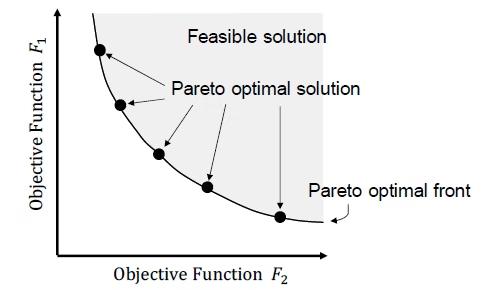
\includegraphics[width=0.4\textwidth]{ParetoFront}
        \caption{Pareto边界示意图}
        \label{fig:pf}
    \end{figure}

    \subsection{多目标进化算法与分类}
    \textbf{多目标进化算法(Multi-objective Evolutionary Algorithm,简称MOEA)}是一种非常有效的解决多目标优化问题(MOP)的方法。1989年,David Goldberg在其著作《Genetic Algorithm in Search, Optimization and Machine Learning\parencite{goldberg1989genetic}》中,提出了用进化算法实现多目标的优化技术,对多目标进化算法的研究具有重要的方向性指导意义。根据不同的进化机制,MOEA可以分为三类\parencite{郑金华2017多目标进化优化}:
    \begin{enumerate}
        \item 基于分解的MOEA:权重聚合函数、切比雪夫聚合、基于惩罚的边界交叉、MOEA/D
        \item 基于支配关系的MOEA:NSGA-II、NPGA、SPEA2、PESA、PAES、MOMGA、mBOA、MMOGA
        \item 基于指标的MOEA:SMS-EMOA、IBEA、HypE
    \end{enumerate}

    \subsection{NSGA-II算法}
    1994年,Srinivas和Deb提出了NSGA(nondominated sorting genetic algorithm)\parencite{NSGA},可以有效求解MOP问题,但仍存在一些不足之处:(1)缺少最优个体保留机制(2)共享参数大小不易确定(3)构造非支配集的时间复杂度高$(O(rN^3))$。2000年,Deb等对算法进行优化,提出了NSGA-II\parencite{NSGA2prototype},2002年又对其中的非支配集排序方法进行了改进\parencite{NSGA2},把时间复杂度提高到$(O(rN^2))$,但只适用于处理低维优化问题(维数小于等于3)。2013年,Deb等又提出了NSGA-III\parencite{NSGA3},用以解决高维数问题。

    本文主要集中讨论NSGA-II算法。

    \section{NSGA-II算法原理及框架}
    \subsection{算法框架}
    NSGA-II算法是一种多目标进化算法,全称是Elitist Non-dominated Sorting Genetic Algorithm(精英非支配排序遗传算法),NSGA-II的主要特征有三点:
    \begin{itemize}
        \item 基于快速非支配排序的等级(rank)划分方法
        \item 计算拥挤度(crowding-distance)的方法
        \item 用以上二者构建的偏序比较算子代替共享参数(sharing fuction)
    \end{itemize}

    NSGA-II算法基于遗传算法的逐代进化思想,开始时随机产生一个父代种群$P_t$,然后利用选择、交叉、变异的方式生成临时子代$Q_t$,利用“非支配排序”与“拥挤度计算”来对父子种群中的每个个体进行适应度评估,选出新一代的n个个体作为新的父代$P_{t+1}$,如此不断循环进化,直到满足结束条件。

    NSGA-II基本流程框架如\figref{fig:nsga-ii-structure}所示:
    \begin{figure}[!h]
        \centering
        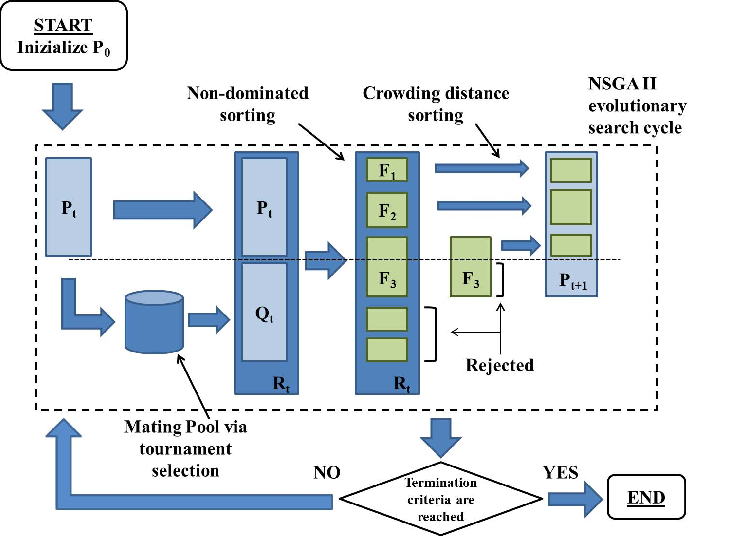
\includegraphics[width=0.5\textwidth]{nsga-ii-stucture}
        \caption{NSGA-II流程示意图}
        \label{fig:nsga-ii-structure}
    \end{figure}

    \subsection{快速非支配集排序方法}
    在NSGA中,非支配集排序方法的时间复杂度是$(O(rN^3))$,NSGA-II改进了非支配集的构造方式,进化群体F中的第2个个体只需要1次比较操作,F中的第3个个体最多只需要2次比较,以此类推,F中第N个个体最多只需要(N-1)次比较操作。在最坏情况下,即当尸中所有个体均为非支配个体时,算法的比较操作总次数为
    $$1+2+3+\dots+(N-1)=N^2/2$$

    考虑到每次比较时有r个子目标,因此,算法的时间复杂度为$O(rN^2)$。
    \begin{figure}[!h]
        \centering
        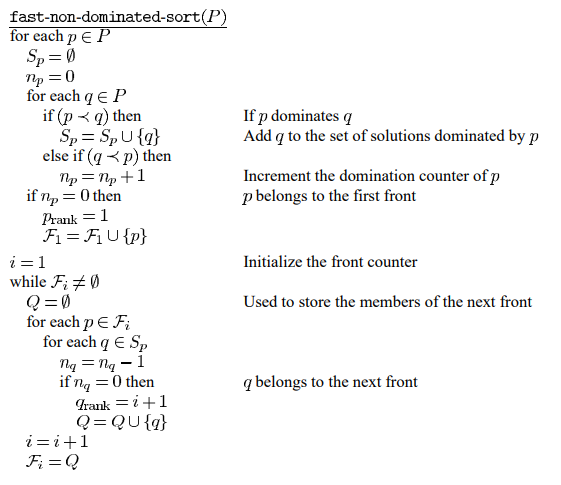
\includegraphics[width=0.7\textwidth]{fast-non-dominated-sort}
    \end{figure}

    \subsection{拥挤度计算方法}
    设下标为i的个体的拥挤度记为$i_{distance}$,目标函数值记为$f_k(x_i)$,用$f_k^{max}$与$f_k^{min}$分别表示目标函数的最大最小值,则拥挤度计算可使用以下公式:

    边界上的点:$i_{distance}=\infty$

    边界以外的点:$i_{distance}= \sum\limits_{k=1}^r(\dfrac{f_k(x_{i+1}) - f_k(x_{i-1})}{f_k^{max} - f_k^{min}})$

    为了计算个体的拥挤度,需要按每个子目标函数值进行排序,最坏情况下对r个子目标进行排序的时间复杂度为$O(rN\log N)$,而计算拥挤度本身的时间为$O(rN)$,所以此算法的时间复杂度为$O(rN\log N)$。

    \begin{figure}[!h]
        \centering
        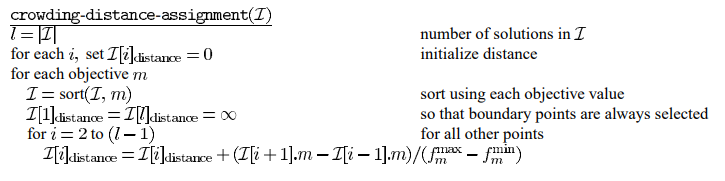
\includegraphics[width=0.9\textwidth]{crowding-distance}
    \end{figure}

    \subsection{精英保留策略}
    NSGA-II的适应度评估过程中,考虑了个体i的两个属性,非支配排序等级与拥挤度,记作$i_{rank}$与$i_{distance}$,二者可以构成一个偏序关系$\prec_n$。

    \begin{definition}
        个体之间的偏序关系$\prec_n$\\
        $$i\prec_nj\ if(i_{rank}<j_{rank}) or ((i_{rank}=j_{rank}) and (i_{distance} > j_{distance}))$$
    \end{definition}
    利用该偏序关系,可以构建偏序比较算子,该算子避免了任何用户定义的参数,同时改善了计算复杂度,有效地保护了多样性。
    精英保留策略1.首先将父代种群C;和子代种群D:合成种群R:。2.根据以下规则从种群见生成新的父代种群Ci+1:
    ①根据Pareto等级从低到高的顺序,将整层种群放入父代种群C,-1,直到某一层该层个体不能全部放入父代种群C:-1;②将该层个体根据拥挤度从大到小排列,依次放入父代种群C+1中,直到父代种群C+1填满。

    \section{算法步骤及实现}

    \subsection{基本步骤}
    以fast-non-dominated-sort()表示非支配排序,以crowding-distance-assignment()表示拥挤度计算,以$Sort(F_i,\prec_n)$表示基于偏序关系$\prec_n$进行适应度排序,则NSGA-II主循环算法可用伪代码描述如下:\\
    \begin{figure}[!h]
        \centering
        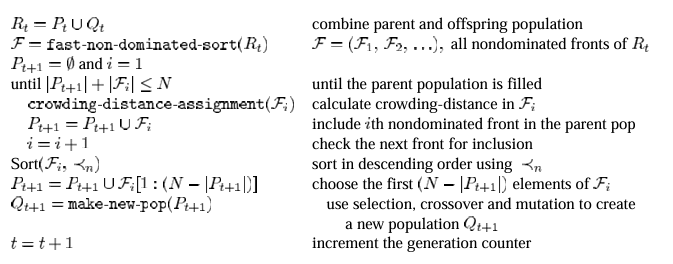
\includegraphics[width=0.8\textwidth]{nsga-ii-algorithm}
    \end{figure}

    具体来说,NSGA-II使用快速非支配排序来保证收敛性,并且利用拥挤距离来保证分布性。

    \subsection{参数设置}
    NSGA-II算法的参数设置对算法的性能有重要影响。主要参数包括:
    \begin{itemize}
        \item 种群规模(N):控制种群中个体的数量。较大的种群规模可以提供更广泛的搜索空间,但计算成本更高。
        \item 最大进化代数(MaxGen):控制算法运行的代数。较大的最大进化代数可以提高算法的收敛性,但计算成本也更高。
        \item 交叉概率(Pc):控制交叉算子应用的概率。较高的交叉概率可以促进种群多样性,但可能导致过早收敛。
        \item 变异概率(Pm):控制变异算子应用的概率。较高的变异概率可以引入新的个体,但可能破坏种群的收敛性。
    \end{itemize}

    \subsection{开源实现}

    \begin{enumerate}
        \item[C]nsga2: https://www.iitk.ac.in/kangal/codes.shtml
        \item[Java]MOEA Framework:https://github.com/MOEAFramework/MOEAFramework
        \item[Python]pymooo: https://github.com/anyoptimization/pymoo
        \item[Julia]Metaheuristics: https://github.com/jmejia8/Metaheuristics.jl
        \item[R]rmoo: https://github.com/Evolutionary-Optimization-Laboratory/rmoo
        \item[Rust]Optirustic: https://github.com/s-simoncelli/optirustic
        \item[C\#]MOEAs: https://github.com/qshzhang/MOEAs
    \end{enumerate}

    可见,NSGA-II算法作为多目标优化(MOO)领域的经典算法,被众多编程语言予以实现,方便后人研究与改进。
    \section{算法应用}
    NSGA-II算法应用非常广泛,

    \subsection{工程设计优化}

    工程设计优化是NSGA-II算法最常见的应用领域之一。在工程设计中,往往需要同时考虑多个目标,如成本、性能、可靠性等。NSGA-II算法可以有效地处理多目标优化问题,找到满足所有目标约束的最佳解决方案。

    案例:飞机机翼设计优化

    飞机机翼设计是一个典型的多目标优化问题,需要同时考虑机翼的升力、阻力、重量等多个目标。使用NSGA-II算法对飞机机翼进行优化,可以找到满足升力、阻力、重量约束的最佳机翼形状。
    逻辑分析:

    定义目标函数:计算飞机机翼的升力和阻力。
    定义NSGA-II算法:包含初始化种群、迭代优化、选择操作、交叉和变异操作等步骤。
    拥挤度计算:计算种群中个体的拥挤度,用于选择操作。
    交叉操作:对两个父个体进行交叉,生成两个子个体。
    变异操作:对个体进行变异,引入多样性。
    运行NSGA-II算法:迭代优化,找到最优解。
    输出最优解:打印飞机机翼的最佳形状。

    \subsection{资源分配优化}

    资源分配优化是NSGA-II算法的另一个重要应用领域。在资源分配问题中,需要在有限的资源约束下,将资源分配给多个任务或项目,以最大化整体收益或最小化成本。NSGA-II算法可以有效地解决此类问题,找到满足资源约束的最佳分配方案。

    案例:项目组合优化

    项目组合优化是一个典型的资源分配优化问题,需要在有限的预算约束下,选择一组项目进行投资,以最大化投资回报率。使用NSGA-II算法对项目组合进行优化,可以找到满足预算约束的最佳项目组合。

    NSGA-II算法在风力发电机组优化中得到了广泛的应用。风力发电机组优化涉及到多目标,如发电量最大化、成本最小化和环境影响最小化。

    应用步骤:

    定义目标函数:
    %
    %发电量:P = 0.5 * ρ * A * V^3 * C_p
    %成本:C = C_i + C_o * P
    %环境影响:E = N_b * P
    %其中,ρ为空气密度,A为叶片面积,V为风速,C_p为功率系数,C_i为初始成本,C_o为运行成本,N_b为噪声水平。

    \subsection{数据挖掘优化}
    数据挖掘优化是NSGA-II算法的又一应用领域。在数据挖掘中,需要从大量数据中提取有价值的信息,如模式、规则或分类器。NSGA-II算法可以优化数据挖掘算法的参数,以提高挖掘效率和准确性。

    案例:特征选择优化

    特征选择是数据挖掘中的一个重要步骤,需要从原始数据集中选择最具区分性的特征。使用NSGA-II算法对特征选择进行优化,可以找到满足分类或回归任务要求的最佳特征子集。


    \nocite{*}
    \printbibliography[heading=bibintoc, title=\ebibname]
\end{document}
